\chapter{Sprites}

In addition to bitmaps and tiles, the \jr\ provides support for sprites, which are mobile graphical objects that can appear anywhere on the screen. \jr\ sprites are similar to the sprites on the Commodore 64 or player-missile graphics on the 8-bit Atari computers, but they are more flexible than either of those. A sprite is essentially a little bitmap that can be positioned anywhere on the screen. Each one can come in one of four sizes: $8 \times 8$, $16 \times 16$, $24 \times 24$, or $32 \times 32$. Each one can display up to 256 colors, picked from one of the four graphics color lookup tables.

A program for the \jr\ can use up to 64 sprites, each one of which is controlled by a block of sprite control registers. The sprite control registers are in I/O page 0, and start at 0xD900. Each sprite takes up 8 bytes, so sprite 0 starts at 0xD900, sprite 1 starts at 0xD908, sprite 2 at 0xD910, and so on. The registers for each sprite are arranged within that block of 8 bytes as shown in table~\ref{tab:sp_reg}.

\begin{table}[h]
    \begin{center}
        \begin{tabular}{|c|c|c|c|c|c|c|c|c|c|c|} \hline
            Offset & R/W & Name & 7 & 6 & 5 & 4 & 3 & 2 & 1 & 0 \\ \hline\hline
            0 & W & Sprite Control & --- & \multicolumn{2}{|c|}{SIZE} & \multicolumn{2}{|c|}{LAYER} & \multicolumn{2}{|c|}{LUT} & ENABLE \\ \hline
            1 & W & \multirow{3}{*}{Sprite Address} & AD7 & AD6 & AD5 & AD4 & AD3 & AD2 & AD1 & AD0 \\ \cline{1-2}\cline{4-11}
            2 & W &  & AD15 & AD14 & AD13 & AD12 & AD11 & AD10 & AD9 & AD8 \\ \cline{1-2}\cline{4-11}
            3 & W &  & \multicolumn{6}{|c|}{---} & AD17 & AD16 \\ \hline
            4 & W & \multirow{2}{*}{Sprite X} & X7 & X6 & X5 & X4 & X3 & X2 & X1 & X0 \\ \cline{1-2}\cline{4-11}
            5 & W &  & X15 & X14 & X13 & X12 & X11 & X10 & X9 & X8 \\ \hline
            6 & W & \multirow{2}{*}{Sprite Y} & Y7 & Y6 & Y5 & Y4 & Y3 & Y2 & Y1 & Y0 \\ \cline{1-2}\cline{4-11}
            7 & W &  & Y15 & Y14 & Y13 & Y12 & Y11 & Y10 & Y9 & Y8 \\ \hline
        \end{tabular}
    \end{center}
    \caption{Sprite Registers for a Single Sprite}
    \label{tab:sp_reg}
\end{table}
These registers manage seven fields:

\begin{description}
    \item[ENABLE] if set, this particular sprite will be displayed (assuming the graphics and sprite engines are enabled in the Vicky Master Control Register).

    \item[LUT] selects the graphics color lookup table to use in assigning colors to pixels

    \item[LAYER] selects which sprite layer the sprite will be displayed on

    \item[SIZE] selects the size of the sprite (see table~\ref{tab:sp_sizes})

    \item[AD] the address of the bitmap (must be within the first 256 KB of RAM). The address is based on the 24-bit system bus, not the CPU's address space.

    \item[X] the X coordinate where the sprite will be displayed (corresponds to the sprite's upper-left corner)

    \item[Y] the Y coordinate where the sprite will be displayed (corresponds to the sprite's upper-left corner)
\end{description}

\begin{table}[h]
    \begin{center}
        \begin{tabular}{|c|c|c|} \hline
            \multicolumn{2}{|c|}{SIZE} & Meaning \\ \hline\hline
            0 & 0 & $32 \times 32$ \\ \hline
            0 & 1 & $24 \times 24$ \\ \hline
            1 & 0 & $16 \times 16$ \\ \hline
            1 & 1 & $8 \times 8$ \\ \hline
        \end{tabular}
    \end{center}
    \caption{Sprite Sizes}
    \label{tab:sp_sizes}
\end{table}

\section{Sprite, Layers, and Display Priority}

While a sprite can be assigned to any of four layers, this layer is only used for determining how the sprite interacts with bitmap or tile map graphics and not how sprites layer with each other. When sprites ``collide,'' a built-in sprite priority order is used to determine which sprite determines a pixel's color. When two sprites are both trying to set the color of a pixel on the screen, the sprite with the lowest number is the one that determines the color. For example, if sprite 0 and sprite 5 are in the same location, it is sprite 0 that will display in the foreground. The sprite layers {\em cannot} be used to change this.

The best practice for assigning sprites is to place the images that need to be on top in the first sprites and those that need to be in the back in the higher numbered sprites. Use the LAYER field for the sprites to control how the sprites layer with the tile maps and bitmaps.

\section{Sprite Positioning}

The coordinate system for sprites is similar to that for bitmap graphics, but it is offset by 32 pixels in both the horizontal and vertical directions. There is a sort of margin area around the entire displayed screen that a sprite can be in and be either partially or completely hidden from view. The horizontal coordinate for a sprite ranges from 0 to 352. The vertical coordinate can range from 0 to 232 or 272, depending on the vertical resolution. For a sprite to have its top-left corner in the top-left of the screen, its position would need to be $(32, 32)$. This coordinate system is the same for all sprites, regardless of their size. Figure:~\ref{fig:sprite_positions} shows how the coordinate system is arranged.

\begin{figure}
    \begin{center}
        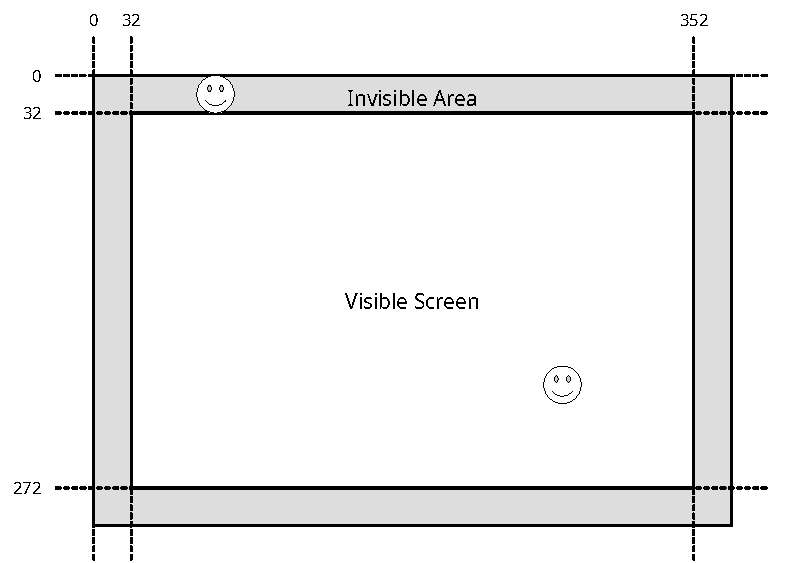
\includegraphics{images/SpritePositions.pdf}
    \end{center}
    \caption{Sprite Positions}
    \label{fig:sprite_positions}
\end{figure}

\example{Displaying a Sprite}
In this example, we'll just put a ball on the screen. First, the program needs to set up TinyVicky to be in sprite mode with no border and a light purple background:

\begin{verbatim}
MMU_IO_CTRL = $0001             ; MMU I/O Control Register

VKY_MSTR_CTRL_0 = $D000         ; Vicky Master Control Register 0
VKY_MSTR_CTRL_1 = $D001         ; Vicky Master Control Register 1
VKY_BRDR_CTRL = $D004           ; Vicky Border Control Register
VKY_BKG_COL_B = $D00D           ; Vicky Graphics Background Color Blue Component
VKY_BKG_COL_G = $D00E           ; Vicky Graphics Background Color Green Component
VKY_BKG_COL_R = $D00F           ; Vicky Graphics Background Color Red Component

VKY_SP0_CTRL = $D900            ; Sprite #0's control register
VKY_SP0_AD_L = $D901            ; Sprite #0's pixel data address register
VKY_SP0_AD_M = $D902
VKY_SP0_AD_H = $D903
VKY_SP0_POS_X_L = $D904         ; Sprite #0's X position register
VKY_SP0_POS_X_H = $D905
VKY_SP0_POS_Y_L = $D906         ; Sprite #0's Y position register
VKY_SP0_POS_Y_H = $D907

            ;
            ; Set up TinyVicky to display sprites
            ;
            lda #$24                    ; Graphics and Sprite engines enabled
            sta VKY_MSTR_CTRL_0
            stz VKY_MSTR_CTRL_1         ; 320x240 @ 60Hz

            stz VKY_BRDR_CTRL           ; No border

            lda #$96                    ; Background: lavender
            sta VKY_BKG_COL_R
            lda #$7B
            sta VKY_BKG_COL_G
            lda #$B6
            sta VKY_BKG_COL_B
\end{verbatim}

Next, the program loads the sprite's colors into the CLUT (\verb+ptr_src+ and \verb+ptr_dst+ are 16-bit storage locations in zero page and are used as pointers):

\begin{verbatim}
            ;
            ; Load the sprite LUT into memory
            ;

            lda #$01                    ; Switch to I/O Page #1
            sta MMU_IO_CTRL

            lda #<balls_clut_start      ; Set the source pointer to the palette data
            sta ptr_src
            lda #>balls_clut_start
            sta ptr_src+1

            lda #<VKY_GR_CLUT_0         ; Set the destination pointer to Graphics CLUT 1
            sta ptr_dst
            lda #>VKY_GR_CLUT_0
            sta ptr_dst+1

            ldx #0                      ; X is a counter for the number of colors copied
color_loop: ldy #0                      ; Y is a pointer to the component within a CLUT color
comp_loop:  lda (ptr_src),y             ; Read a byte from the code
            sta (ptr_dst),y             ; And write it to the CLUT
            iny                         ; Move to the next byte
            cpy #4
            bne comp_loop               ; Continue until we have copied 4 bytes

            inx                         ; Move to the next color
            cmp #16
            beq done_lut                ; Until we have copied all 16

            clc                         ; Advance ptr_src to the next source color entry
            lda ptr_src
            adc #4
            sta ptr_src
            lda ptr_src+1
            adc #0
            sta ptr_src+1

            clc                         ; Advance ptr_dst to the next destination color entry
            lda ptr_dst
            adc #4
            sta ptr_dst
            lda ptr_dst+1
            adc #0
            sta ptr_dst+1

            bra color_loop              ; And start copying that new color

done_lut:   stz MMU_IO_CTRL             ; Go back to I/O Page 0
\end{verbatim}

Finally, we point sprite 0 to the pixel data (which is included in the assembly code below), set its location on the screen (which will be the upper left corner of the screen), and then we turn on the sprite setting its LUT and LAYER in the process:

\begin{verbatim}
            ;
            ; Set up sprite #0
            ;
init_sp0:   lda #<balls_img_start       ; Address = balls_img_start
            sta VKY_SP0_AD_L
            lda #>balls_img_start
            sta VKY_SP0_AD_M
            stz VKY_SP0_AD_H

            lda #32
            sta VKY_SP0_POS_X_L         ; (x, y) = (32, 32)... should be upper-left corner of the screen
            stz VKY_SP0_POS_X_H

            lda #32
            sta VKY_SP0_POS_Y_L
            stz VKY_SP0_POS_Y_H

            lda #$41                    ; Size = 16x16, Layer = 0, LUT = 0, Enabled
            sta VKY_SP0_CTRL
\end{verbatim}

Here is the pixel data for the sprite:
\begin{verbatim}
balls_img_start:
    .byte $00, $00, $00, $00, $00, $00, $03, $02, $02, $01, $00, $00, $00, $00, $00, $00
    .byte $00, $00, $00, $00, $05, $05, $04, $03, $03, $03, $03, $02, $00, $00, $00, $00
    .byte $00, $00, $00, $07, $07, $07, $06, $05, $04, $04, $03, $03, $01, $00, $00, $00
    .byte $00, $00, $07, $09, $0A, $0B, $0A, $08, $06, $05, $04, $03, $02, $01, $00, $00
    .byte $00, $05, $07, $0A, $0D, $0E, $0D, $0A, $07, $05, $05, $04, $03, $01, $01, $00
    .byte $00, $05, $07, $0B, $0E, $0E, $0E, $0C, $07, $05, $05, $04, $03, $01, $01, $00
    .byte $03, $04, $06, $0A, $0D, $0E, $0D, $0A, $07, $05, $05, $04, $03, $02, $01, $01
    .byte $02, $03, $05, $08, $0A, $0C, $0A, $08, $06, $05, $05, $04, $03, $02, $01, $01
    .byte $02, $03, $04, $06, $07, $07, $07, $06, $05, $05, $05, $04, $03, $01, $01, $01
    .byte $01, $03, $04, $05, $05, $05, $05, $05, $05, $05, $05, $03, $03, $01, $01, $01
    .byte $00, $03, $03, $04, $05, $05, $05, $05, $05, $05, $04, $03, $02, $01, $01, $00
    .byte $00, $02, $03, $03, $04, $04, $04, $04, $04, $03, $03, $02, $01, $01, $01, $00
    .byte $00, $00, $01, $02, $03, $03, $03, $03, $03, $03, $02, $01, $01, $01, $00, $00
    .byte $00, $00, $00, $01, $01, $01, $02, $02, $01, $01, $01, $01, $01, $00, $00, $00
    .byte $00, $00, $00, $00, $01, $01, $01, $01, $01, $01, $01, $01, $00, $00, $00, $00
    .byte $00, $00, $00, $00, $00, $00, $01, $01, $01, $01, $00, $00, $00, $00, $00, $00
\end{verbatim}

Here are the colors for the sprite (note that this example is using only 15 colors, to make the example more understandable in print):
\begin{verbatim}
balls_clut_start:
    .byte $00, $00, $00, $00
    .byte $88, $00, $00, $00
    .byte $7C, $18, $00, $00
    .byte $9C, $20, $1C, $00
    .byte $90, $38, $1C, $00
    .byte $B0, $40, $38, $00
    .byte $A8, $54, $38, $00
    .byte $C0, $5C, $50, $00
    .byte $BC, $70, $50, $00
    .byte $D0, $74, $68, $00
    .byte $CC, $88, $68, $00
    .byte $E0, $8C, $7C, $00
    .byte $DC, $9C, $7C, $00
    .byte $EC, $A4, $90, $00
    .byte $EC, $B4, $90, $00
\end{verbatim}
